\documentclass[a4paper,11pt]{article}

% Packages for additional functionality
\usepackage[utf8]{inputenc} % For UTF-8 encoding
\usepackage{amsmath, amssymb} % For math symbols
\usepackage{hyperref} % For hyperlinks
\usepackage{listings} % For code blocks
\usepackage{xcolor} % For syntax highlighting in code
\usepackage{graphicx}
% Customize hyperlink colors
\hypersetup{
    colorlinks=true,
    linkcolor=blue,
    filecolor=magenta,
    urlcolor=cyan,
}

% Set the default font style
\renewcommand{\familydefault}{\sfdefault}

\newcommand{\doctitle}{Quickstart guide for UniNuvola}
\newcommand{\docsubtitle}{A quickstart guide about how to use UniNuvola paltform and its main feaatures}

% Code block style
\lstset{
    basicstyle=\ttfamily\small,
    backgroundcolor=\color{lightgray},
    frame=single,
    breaklines=true,
    postbreak=\mbox{\textcolor{red}{$\hookrightarrow$}\space},
}

% Document starts
\begin{document}

% frontmatter.tex
\begin{titlepage}
    \thispagestyle{empty}
    \begin{center}
        % Logo
        \vspace*{1.5cm}
        
\includegraphics[width=0.7\textwidth]{img/uninuvola_logo.jpeg} % <-- Replace with your logo

        % Organization Name
        %\vspace{1cm}
        %{\Large \textsc{My Organization Name}} % <-- Replace with your org name

        % Document Title
        \vspace{2.5cm}
        {\Huge \bfseries \doctitle} \\[1ex] % <-- Replace with your title

        % Subtitle (optional)
        {\large \textit{\docsubtitle}} % <-- Replace or remove

        % Author(s)
        \vspace{2.5cm}
        {\large \textbf{The UniNuvola Team}} \\[0.5ex] % <-- Replace with actual names

        % GitHub Issue
        \vspace{2.5cm}
        {\large For any issue please report it using the GitHub page: \href{https://github.com/UniNuvola/UniNuvola}{UniNuvola}}
        % Update Date
        \vfill
        {\normalsize Last Updated: \today} % <-- Or replace \today with a fixed date

        % Footer (optional)
        % TODO: delate or keep ??
        \vspace{1cm}
        {\small © \the\year\ University of Perugia. All rights reserved.} % <-- Update as needed
    \end{center}
\end{titlepage}
\section{Introduction}

Welcome to this quickstart guide for using UniNuvola. This is not a comprehensive manual—one will be made available
soon—but it provides the information required to start using the prototype server.

\section{Accessing the server}

You can access UniNuvola via web browser, using the University VPN, through the
\href{https://www.uninuvola.unipg.it/}{https://www.uninuvola.unipg.it/} website. You will be redirected to the UniNuvola
Vault login page. After selecting the LDAP option (Figure \ref{fig:login}) in the drop-down menu, you can enter your
login details: these are the same as those you use to access the University services (user id and password). If it is
your first time accessing the server, you will be redirected to a web page  where you will automatically request access
to the infrastructure. Access will be granted once one of the operators approves your request (Figure
\ref{fig:pending}). If you already have an account, or after you get accepted you will redirected to the image and
resources selection page.


\begin{figure}[!ht]
    \centering
    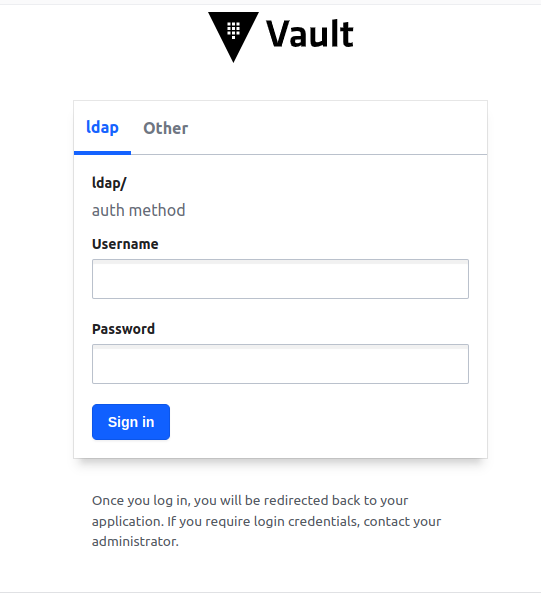
\includegraphics[width=0.5\linewidth]{img/login_page.png}
    \caption{UniNuvola's login page.}
    \label{fig:login}
\end{figure}



\begin{figure}[!ht]
    \centering
    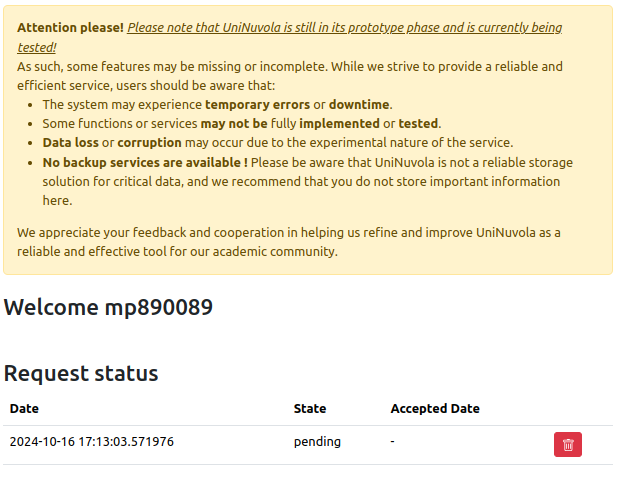
\includegraphics[width=0.5\linewidth]{img/request_page.png}
    \caption{Pending acceptance page}
    \label{fig:pending}
\end{figure}

\section{Selection of the Image and resources}

\textbf{Note:} This section will undergo further modifications within the next month, and the quickstart will be updated
accordingly. \\

After a successful login, you will be directed to the resource selection page. The first section to complete is the
image selection. This part needs to be filled in by the user or select one of the available options. Images can be
selected from those available in UniNuvola (see table \ref{tab:images}) or from your own customised version on
Dockerhub. The tags \textit{latest} and \textit{deployed} are available in our harbor repository.\\

\begin{table}[]
    \caption{List of the official images in UniNuvola}
    \label{tab:images}
    \centering
    \begin{tabular}{|c|c|}
        \hline
        Base              & harbor1.fisgeo.unipg.it/uninuvola/base             \\ \hline
        Engineering       & harbor1.fisgeo.unipg.it/uninuvola/engineering      \\ \hline
        Conda             & harbor1.fisgeo.unipg.it/uninuvola/conda            \\ \hline
        Chemistry         & harbor1.fisgeo.unipg.it/uninuvola/chemistry        \\ \hline
        Quantum Computing & harbor1.fisgeo.unipg.it/uninuvola/quantumcomputing \\ \hline
        Genomics          & harbor1.fisgeo.unipg.it/uninuvola/genomics         \\ \hline
        Hydraulics        & harbor1.fisgeo.unipg.it/uninuvola/hydraulics       \\ \hline
        Tensorflow        & harbor1.fisgeo.unipg.it/uninuvola/tensorflow       \\ \hline
        Pytorch           & harbor1.fisgeo.unipg.it/uninuvola/pytorch          \\ \hline
        Pytorch-GPU       & harbor1.fisgeo.unipg.it/uninuvola/pytorchgpu       \\ \hline
        Optimisation      & harbor1.fisgeo.unipg.it/uninuvola/optimisation     \\ \hline
    \end{tabular}
\end{table}


The image name will appear as:
\begin{lstlisting}[language=bash] 
harbor1.fisgeo.unipg.it/uninuvola/base:deployed
\end{lstlisting}

In the next drop-down menus, you will choose the number of CPUs required (1, 2, 4, 8, 16, 32), the amount of RAM
required (4 Gb, 8 Gb, 16 Gb, 32 Gb), and, if you require GPUs, the number of them (0, 1, 2, 3, 4). At the moment, 100
gigabyte of persistent storage are available for each user (Figure \ref{fig:resources}).\\

\begin{figure}[!ht]
    \centering
    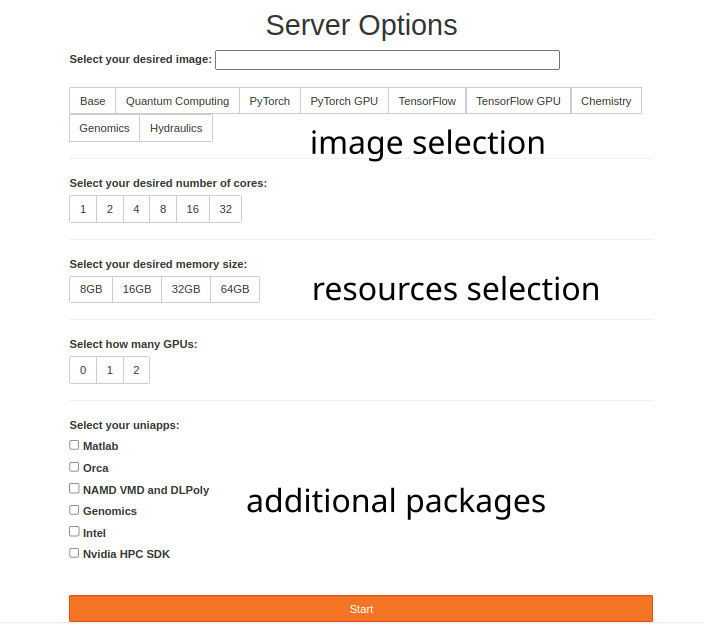
\includegraphics[width=0.75\linewidth]{img/resource_selection.png}
    \caption{Resources selection page}
    \label{fig:resources}
\end{figure}

As per the disclaimer in Figure \ref{fig:pending}, remember: \textbf{UniNuvola is a prototype. We provide computational
    power and storage, but data are not backed up. Be careful with your data!} \\

\section{Inside UniNuvola}
The main page of UniNuvola appears as depicted in Figure \ref{fig:uninuvola_main_page}. The top bar allows some
management actions and some customisation of the user interface. Most importantly, inside the file men, you can find the
disconnect and  the control hub options. The former allows to connect and disconnect from Jupyter (be aware that you
will disconnect from the Hub page, but the pod will continue run up to 12 hours after becoming inactive), the later
option allows to kill the running image and it allows the user to load a new image. \\

the left side of the menu allows the management of the local files. The four most upper options allow the user in order
to: open new launchers tabs, create new directories, upload files, and refresh the browser. Files can be moved through
the web interface or through remote terminal connection from UniNuvola to the machine hosting the files.\\

The orange square includes all Python and R toolkits. The top part includes all the environments notebooks in the image,
the bottom part instead the relative consoles. The top right part, the purple square, contains the Xpra notebook, that
allows the usage of programs requiring a graphical interface.  \\

In the last line, the first element, circled in green, allows the user to use a terminal. All terminals will start with
the sh/bash terminal depending on the image. The elements circled in blue are the text editors in the Hub,  in the case
of the figure a general text editor, a Markdown and a Python file editor. \\


\begin{figure}[!ht]
    \centering
    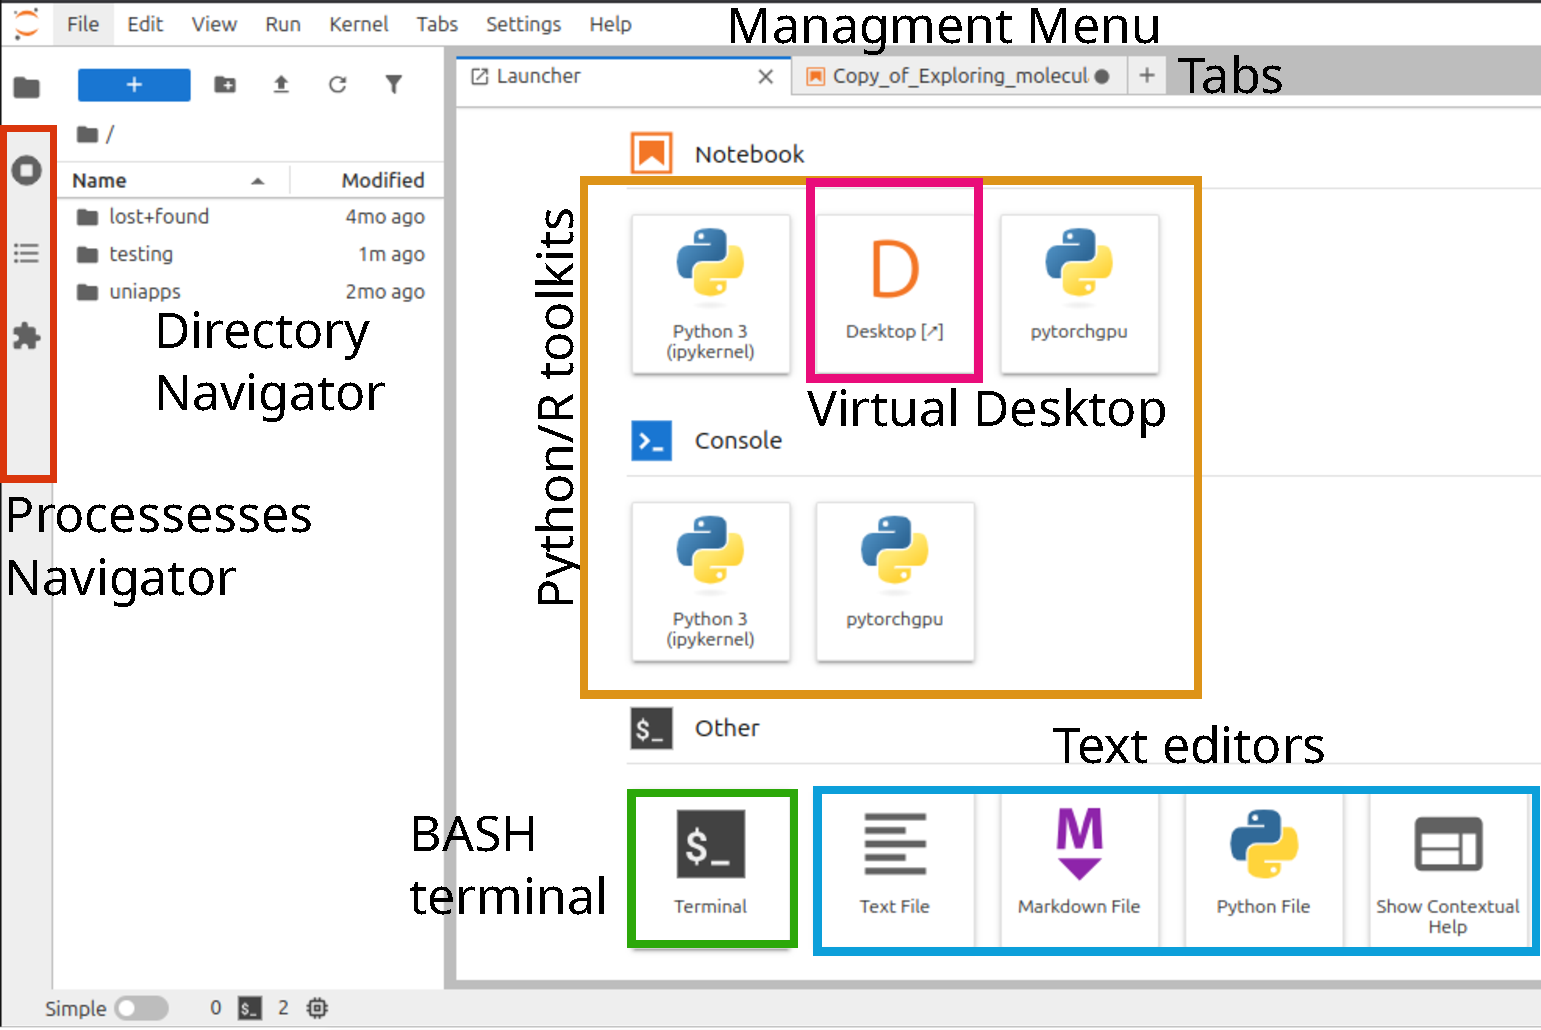
\includegraphics[width=0.8\linewidth]{img/uninuvola.pdf}
    \caption{Example of Jupyter Lab interface in UniNuvola.}
    \label{fig:uninuvola_main_page}
\end{figure}

Each user has the possibility of create 5 Jupyter  named nodes that can be used as scratch space. The option can be
found in the Hub Control Panel into the File menu. Figure \ref{fig:uninuvola_multi} shows an example page.

\begin{figure}[!ht]
    \centering
    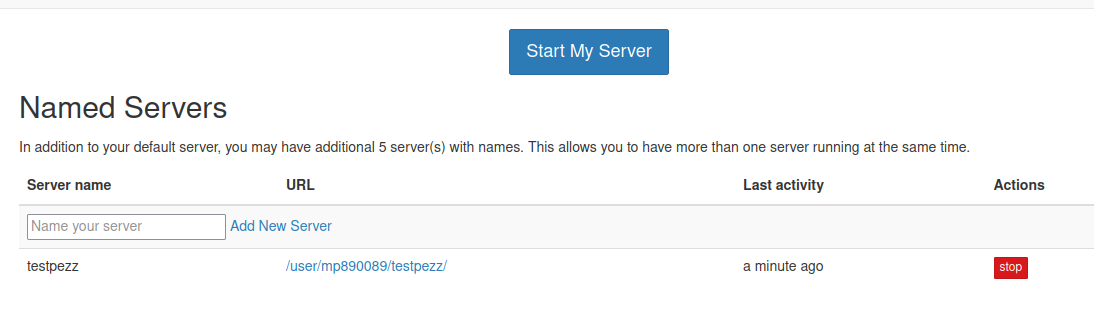
\includegraphics[width=0.90\linewidth]{img/multiserver.png}
    \caption{Named server page example}
    \label{fig:uninuvola_multi}
\end{figure}

\section{Activation of the conda environment}
The first time an user enters in UniNuvola or deletes the .bashrc, conda is not active in the terminal. At this stage
the process can be done manually following these steps:
\begin{lstlisting}[language=bash] 
/opt/conda/condabin/conda  init source ~/.bashrc
\end{lstlisting}
Afterwards, you will be able to use conda as in any other environment.

\section{Troubleshooting}
\subsection{Multiple readdressing into the login page}
If you didn't logout after your account creation, or your token expired, it is possible that in the following session
you can be readdressed into the login page.  In order to solve the issue you can opt for two solutions:
\begin{itemize}
    \item[\textbf{I}] disconnect by hand from the UniNuvola Vault page.
    \item[\textbf{II}] delete the cookies in your browser.
\end{itemize}

To achieve the fist step, you will need to connect to the
\href{https://vault.uninuvola.unipg.it:8200/ui/vault/dashboard}{UniNuvola Vault webpage}, press on the icon representing
a person and than click logout. Figure \ref{img:logout} shows the process.      \\
\begin{figure}[!h]
    \center
    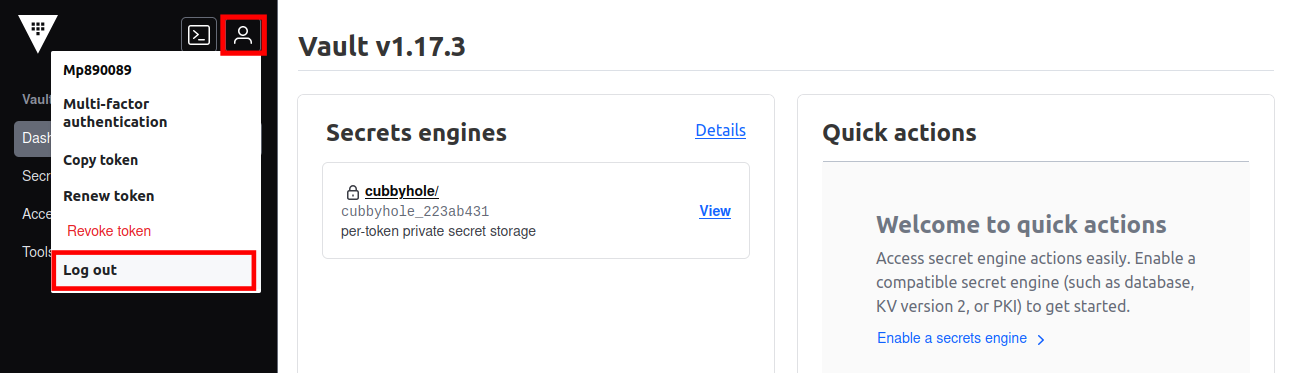
\includegraphics[width=0.8\linewidth]{img/vault.png}
    \caption{Uninvola's Vault logout page.}
    \label{img:logout}
\end{figure}

Afterwards you should be able to reaccess to UniNuvola.


\end{document}
